\documentclass[ignorenonframetext,10pt]{beamer}

%\usepackage[latin1]{inputenc}
\usepackage[english]{babel}
\usepackage{amsmath,amssymb}
\usepackage{multimedia}
\usepackage{alltt}
\usepackage{multirow}
\usepackage{textcomp}
\usepackage[footnotesize]{subfigure}
\usepackage{graphicx}


%\usetheme{Berlin}
\usetheme{Darmstadt}
\useoutertheme[subsection=false]{miniframes}
\useoutertheme{smoothbars}
\usefonttheme{structurebold}
%\setbeamertemplate{navigation symbols}{}
\setbeamercovered{invisible}


\title{Helices of RNAs}
\author{\large Jiabin~Huang}
\date{\today}

\institute[ExpBI]{\normalsize
  AG Experimentelle Bioinformatik (Cyanolab)\\
  Institut f\"ur Biologie III\\
  Universit\"at Freiburg}
  
  


\begin{document}

\frame{\maketitle}


\begin{frame}
\frametitle{Outline}
   \begin{itemize}
   \item Introduction
   \item Development of a new structure abstraction
   \item Implementation of an algorithm based on the new abstraction
   \item Possible problems              
   \item Evaluation of the algorithm
   \item Designing RNA class predictors   
   \end{itemize}
\end{frame}


\section{Introduction}
\subsection{}
\begin{frame}
\frametitle{Structural components of RNA}
  %\begin{block}
   RNA has different structural components:
   \begin{itemize}
   \item single-stranded regions (SS)
   \item hairpin loops (HL)
   \item stacking regions (SR)
   \item bulges on 5\'{}side (BL) or 3\'{}side (BR)
   \item internal loops (IL)
   \item multiloops (ML). 
   \end{itemize}
  %\end{block}
\end{frame}
  
\begin{frame}
\frametitle{Structural components of RNA}  
\begin{figure}
  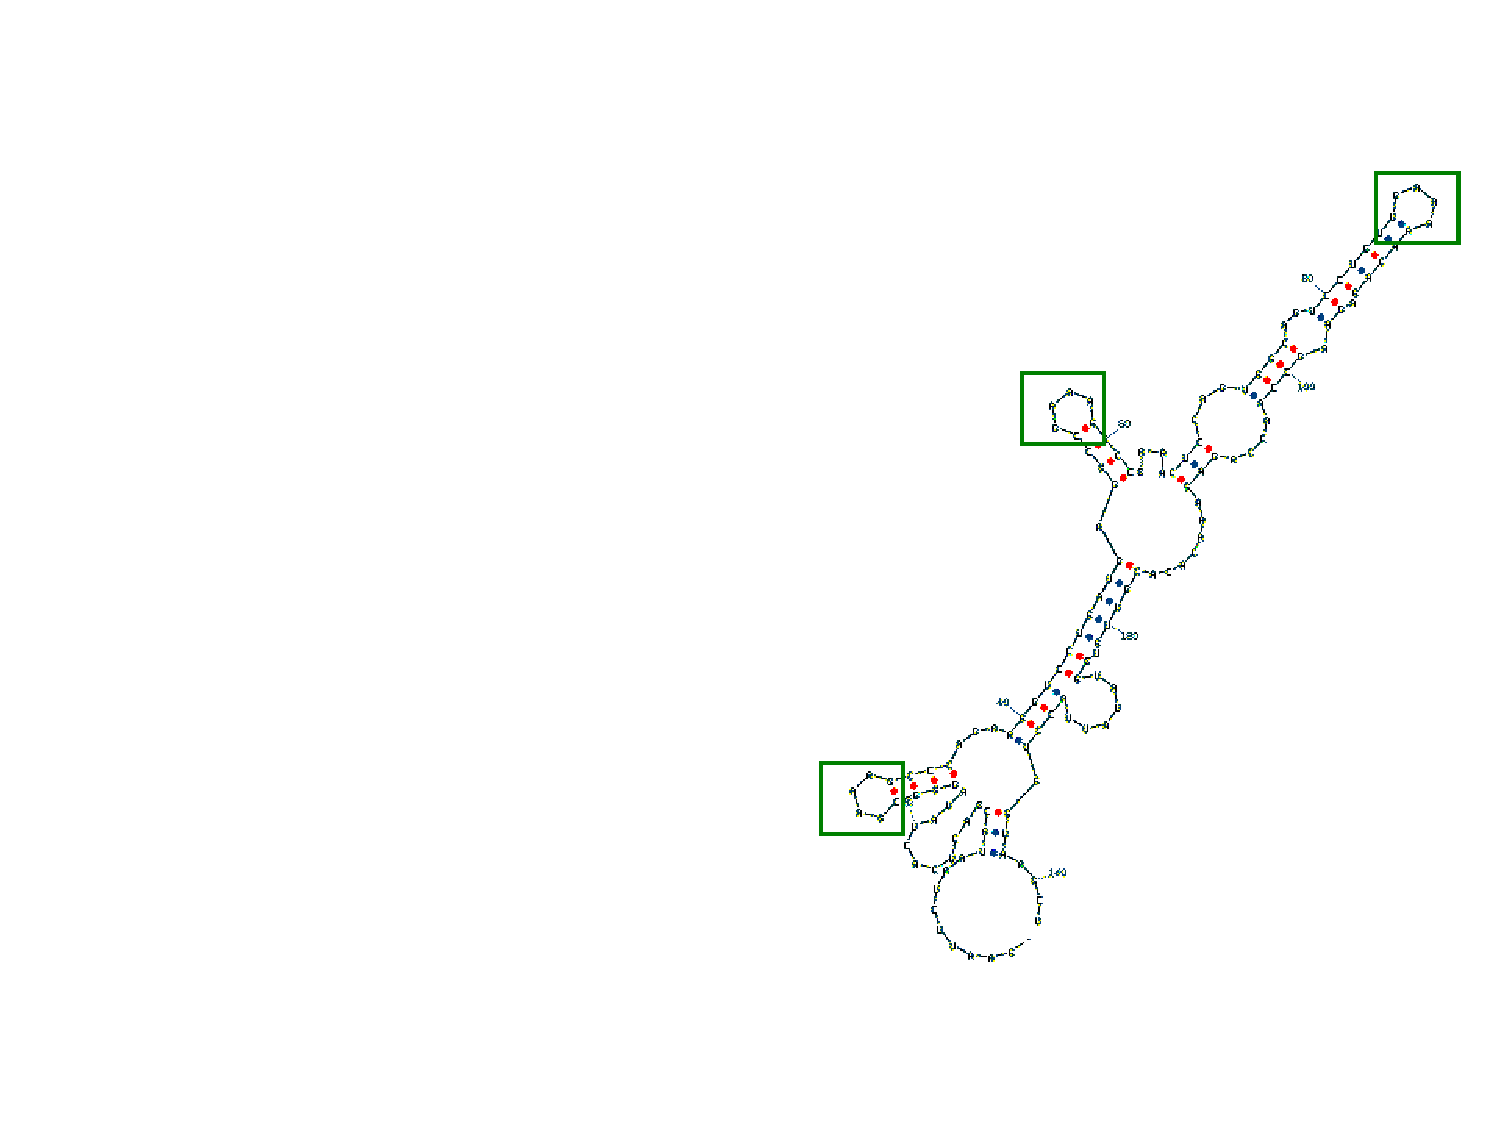
\includegraphics[scale=0.4]{images/structural_components.pdf} 
  \caption{Structural components}
\end{figure}
\end{frame}

% \frame{
%   \frametitle{tRNAs - Proof of Correctness}
%   \begin{block}{Alignment and Predicted Consensus}
%     \begin{figure}
%       %\subfigure[Rfam
%       % Alignment]{\includegraphics[width=\textwidth]{images/tRNA_example_ungap_ali_coloured.pdf}}
%       %\subfigure[RNAlishapes]{\includegraphics[width=.3\textwidth]{images/tRNA_example_structure_plot.pdf}}
%       %\hspace{2cm}
%       %\subfigure[RNAalifold]{\includegraphics[width=.3\textwidth]{images/tRNA_example_structure_plot.pdf}}
%     \end{figure}
%   \end{block}
% }


\begin{frame}
\frametitle{Visualisation of structures}  
\begin{figure}
  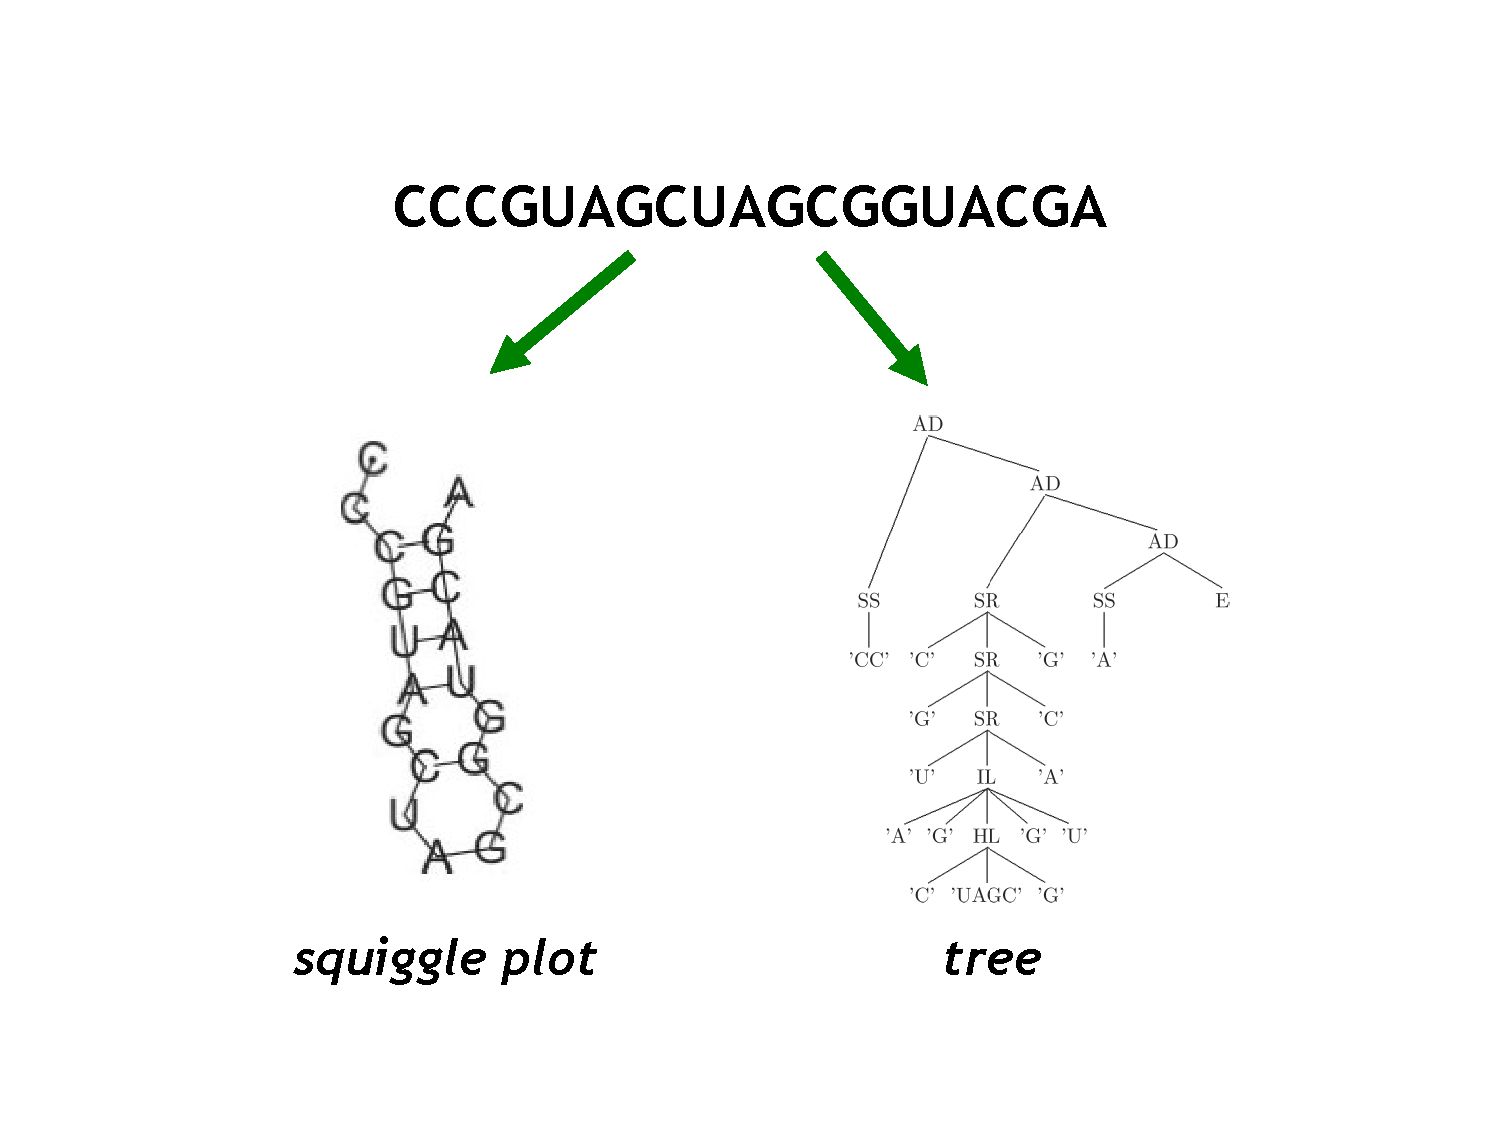
\includegraphics[scale=0.4]{images/visualisation_structures.pdf} 
  %\caption{Structural components}
\end{figure}
\end{frame}

\begin{frame}
\frametitle{Suboptimal structures}
%\pause
   \begin{itemize} 
   \item But the \'84true`` structure is not always the one with
   \item the lowest predicted free energy.
   \end{itemize}
\end{frame}

\begin{frame}
\frametitle{Introducing abstract shapes}
%\pause
   \begin{itemize} 
   \item Solution: Use abstract shapes to describe a set of structures.
   \end{itemize}
\end{frame}

\begin{frame}
\frametitle{Introducing abstract shapes}
%\pause
   \begin{itemize} 
   \item In the domain of shapes, we care only about
   \item open structures (OP)
   \item closed structure (CP)
   \item branching (``fork'', FK) and
   \item adjacency of structures (AD).
   \end{itemize}
\end{frame}

\begin{frame}
\frametitle{Defining abstract shapes}
%\pause
   \begin{itemize} 
   \item A (very abstract) abstraction function :
   \item $\pi$(SS(l))           = OP      (single-stacked region)
   \item $\pi$(HL(a,l,b)         = CL      (hairpin)
   \item $\pi$(SR(a,x,b))       = $\pi$(x)                       (stacked region)
   \item $\pi$(IL(a,l,x,l\'b4,b))  = \'f0(x)       (interior loop)
   \item $\pi$(ML(a,c,b))       = FK($\pi$(x))                (multiloop) 
   \item E represents the ``empty structure''.
   \item where a, b = nucleotides, l = loop, c = list of adjacent 
   \item components and x = arbitrary structure elements.
   \end{itemize}
\end{frame}






\section{2}
\subsection{}
\begin{frame}
\frametitle{Example }
%\pause
\end{frame}

\begin{frame}
\frametitle{Computing abstract shapes}
%\pause
   \begin{itemize} 
   \item Abstract shapes are a homomorphic image of the folding
   \item space of a RNA sequence (same as mfe or base pair 
   \item maximization).
   \item They can therefore be computed using Dynamic
   \item Programming (DP).  
   \item Giegerich et al. use an extension of DP called
   \item Algebraic Dynamic Programming (ADP).
   \item ADP offers some interesting aspects (separation of
   \item recognition and evaluation, pair algebras).
   \end{itemize}
\end{frame}

\begin{frame}
\frametitle{Computing abstract shapes}
%\pause
   \begin{itemize} 
   \item  \emph{Algebraic Dynamic Programming} defines the set of all possible solutions (e.g. foldings) using a context-free grammar.
   \end{itemize}
\end{frame}

\begin{frame}
\frametitle{First summary  }
%\pause
   \begin{itemize} 
   \item  One abstract shape represents a family of  
   \item     similar RNA structures.
   \item Shapes are defined by an abstraction function
   \item    that maps from structure to shape space.
   \item Shapes can be used to represent a large number of (suboptimal) foldings to obtain an holistic view of the folding space.
   \end{itemize}
\end{frame}

\begin{frame}
\frametitle{Applications of abstract shapes}
%\pause
   \begin{itemize} 
   \item Suboptimal Folding
   \item Out of 99 tRNA sequences in Rfam only 30 had the typical cloverleaf structure as predicted mfe folding.
   \item Example: tRNA of  \emph{Natronobacterium pharaonis:}
   \item  \emph{    }mfe structure is a hairpin with internal loops, cloverleaf structure occurs at position 104 of 199 
   \item     suboptimal structures.
   \item All these suboptimal folding can be represented by three abstract shapes.
   \end{itemize}
\end{frame}

\begin{frame}
\frametitle{Applications of abstract shapes}
%\pause
   \begin{itemize} 
   \item Suboptimal Folding
   \item (demo)
   \end{itemize}
\end{frame}

\begin{frame}
\frametitle{Applications of abstract shapes}
%\pause
\end{frame}

\begin{frame}
\frametitle{Suboptimal folding}
%\pause
\end{frame}

\begin{frame}
\frametitle{Applications of abstract shapes}
%\pause
   \begin{itemize} 
   \item Better structure prediction (than mfe folding) can
   \item be obtained using comparative approaches:
   \end{itemize}
\end{frame}

\begin{frame}
\frametitle{Applications of abstract shapes}
%\pause
   \begin{itemize} 
   \item A possible resort : 
   \end{itemize}
\end{frame}






\section{3}
\begin{frame}
\frametitle{Applications of abstract shapes}
%\pause
   \begin{itemize} 
   \item Consensus structures with abstract shapes
   \end{itemize}
\end{frame}

\begin{frame}
\frametitle{Applications of abstract shapes}
%\pause
   \begin{itemize} 
   \item Possible scoring functions:
   \end{itemize}
\end{frame}

\begin{frame}
\frametitle{Going comparative pays off}
%\pause
\end{frame}

\begin{frame}
\frametitle{Comparison with Sankoff}
%\pause
\end{frame}

\begin{frame}
\frametitle{Summary }
%\pause
   \begin{itemize} 
   \item Abstract shapes represent disjoint classes of RNA foldings.
   \item Shapes are computed using (Algebraic) Dynamic Programming.
   \item Inspecting the abstract shape space of a sequence
   \item    can give a quick overview of the folding space.
   \item Consensus folding with abstract shapes performs well.
   \item Choice of best abstraction function and energy range 
   \item     is important but difficult.
   \end{itemize}
\end{frame}

\begin{frame}
\frametitle{Conclusions and Outlook}
%\pause
   \begin{itemize} 
   \item Other approaches to suboptimal folding exist such as statistical sampling of the folding space.
   \item Text representations of shapes could be used as index in structure databases to classify non-coding RNA.
   \item Extensions to the shape formalisms are under work
   \item   ( e.g. computation of shape probabilities, de novo prediction of non-coding RNA genes )
   \end{itemize}
\end{frame}

\begin{frame}
\frametitle{End}
%\pause
   \begin{itemize} 
   \item Thanks a lot for your attention !
   \item Questions ?
   \end{itemize}
\end{frame}


\end{document}
